\documentclass[letterpaper]{aamas2009}
%\usepackage{ijcai09}
\usepackage{amssymb}
\usepackage[english]{babel}
\usepackage{latexsym}
\usepackage{amsfonts}
\usepackage{amsmath}
\usepackage{graphicx}
\usepackage{algorithmic}
\usepackage{times}
\usepackage{subfigure}
%\usepackage{natbib}
%
\def\sharedaffiliation{%
\end{tabular}
\begin{tabular}{c}}
%

\numberofauthors{3} 

\author{\alignauthor Zinovi Rabinovich\\
  \affaddr{Electronics and Computer Science}\\
  \affaddr{University of Southampton}\\
  \affaddr{Southampton, United Kingdom}\\
  \email{zr@ecs.soton.ac.uk}
\alignauthor Lachlan Dufton\\ 
  \affaddr{Cheriton School of Computer Science}\\
  \affaddr{University of Waterloo}\\
  \affaddr{Waterloo, Canada}\\
  \email{ltdufton@cs.uwaterloo.ca}
\alignauthor Kate Larson\\
  \affaddr{Cheriton School of Computer Science}\\
  \affaddr{University of Waterloo}\\
  \affaddr{Waterloo, Canada}\\
  \email{klarson@cs.uwaterloo.ca}
} 

\title{Policy  Teaching by a Modulation of the Transition Model}

\begin{document}

\maketitle

\section{Intuition}
Given a learner that attempts to find an action policy to optimise its
utility. We can modify the environment response to the learner's
actions and we want to use this capability to enforce learning of a
particular policy of action.

For instance, if a learning agent needs to find an optimal racing path
(see Figure~\ref{race_path}), depending on the terrain it may take long
time to explore all options. By making the terrain features more
prominent at several locations a teacher can facilitate faster
learning of the intended cycle.

\begin{figure*}[ht]
{\center 
\subfigure[Passive dynamics]{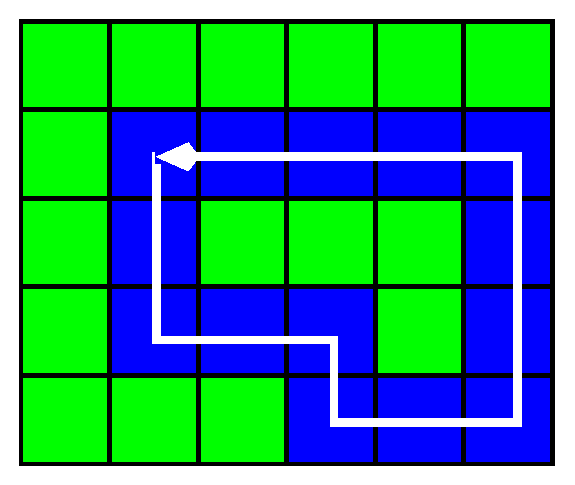
\psfig{file=img/race_track_flat.eps,width=5cm}}
\subfigure[Augmented dynamics]{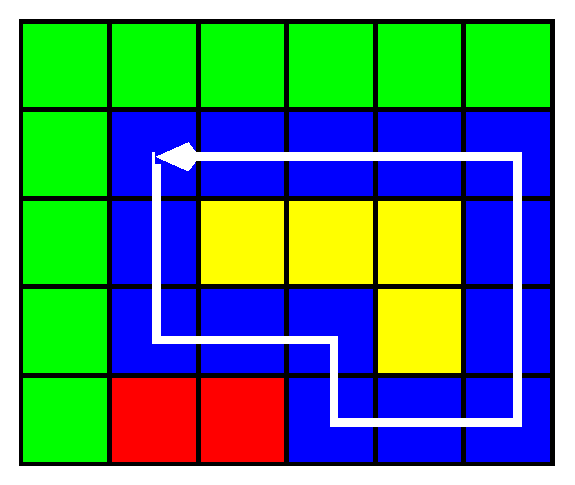
\psfig{file=img/race_track.eps,width=5cm}}\\}
\caption{\label{race_path}Unmodified (passive) and augmented environment dynamics for race path finding (colours naturally encode traversability of the cell)}
\end{figure*}

%We'd like to facilitate learning of a specific policy of action by a learner by means of 
%Instead of providing a direct incentive in the form of a reinforcement
%(either by changing the reward function or by direct interaction) we
%would like to vary the environment response. The intuition is as
%follows. Consider a parent trying to teach a child to ride a bike. At
%first the parent will sit the child on a bike with support
%wheels. Once the child learned basic controls, the parent will elevate
%support wheels to provide only partial support in the case the bike
%looses balance. Then the supports are removed entirely. In other
%words, the environment is distorted in a way that makes the problem
%naturally solved by a behaviour generally resembling the desired one,
%and then the distortion is gradually removed, thus refining a
%basically good behaviour closer and closer to the ideal one.

\section{Model}
The environment is described by the tuple $<S,A,U,T>$, where:
\begin{itemize}
\item $S$ is the state space of the problem the learner agent attempts
  to solve (in the case of the race track these would be the cells of
  the map)
\item $A$ is the set of actions available to the learner (e.g. north, south, etc.)
\item $U$ is the space of environment modifications that the teacher can apply
\item $T:S\times A\times U\rightarrow\Delta(S)$ is the probabilistic
  transition function with $T(s'|s,a,u)$ denoting the probability that
  the system state will change from $s$ to $s'$ if the learner applied
  action $a$ and the teacher chose modification $u$.
\begin{itemize}
\item For any $u\in U$ we denote $T_u:S\times A\rightarrow\Delta(S)=P(s',a,u,s)$
\item Exists a neutral teacher action $u^*$, and its associated
  transition function limitation $T^*=T_{u^*}$ is termed {\bf passive
    dynamics}. This would correspond to the teacher not intervening at all.
\end{itemize}
\end{itemize}

The tasks faced by the two agents are encoded differently:
\begin{itemize}
\item {\bf Learner:} The task is the usual one for a stochastic
  controller. Given $c:S\times A\rightarrow\mathbf{R}$, a single step
  cost function, minimise the expected total (discounted) cost
  $\mathbf{E}\left(\sum\gamma^tr_t\right)$. The solution to the
  problem is an action policy $\pi:S\rightarrow\Delta(A)$. To find the
  solution, the learner begins with some policy $\pi_0$ and then, by
  facing the environment $<S,A,T_u,c>$, updates it
  $\pi_{t+1}=F(\pi_t,u)$.
\item {\bf Teacher:} The teacher is given an idealistic policy
  $\pi^*:S\rightarrow\Delta(A)$ that it wants the learner to reach. The task of the teacher is then twofold:
\begin{itemize}
\item Minimise the distance between the policy chosen by the learner and $\pi^*$
\item Minimise the efforts, that is the distance between the augmented dynamics $T_u$ and $T^*$.
\end{itemize}
The problem faced by the teacher is then:
$$
\min\sum\limits_{t=1}^{t_{max}} Cost(u_t,\pi_t)\ \ s.t.\ \ \pi_t=F(\pi_{t-1},u_t)
$$
where $Cost(u_t,\pi_t)$ measure the two factors above
\end{itemize}
\subsection{Teacher's Cost Computation}
As a measure of cost we will use Kullback-Leibler divergence rate
between two processes formed by the application of the teacher's
augmentation $u_t$ and the learner's policy $\pi_t$. More specifically,
consider the stochastic process over the state-action pairs formed by
the application of the learner's policy in the modified environment at
time $t$: \\
\centerline{$
P_t(s',a'|s,a)=T_{u_t}(s'|s,a)\pi_t(a'|s')
$}

Similarly, denote $P^*(s',a'|s,a)=T^*(s'|s,a)\pi^*(a'|s')$.

The process $P_t$ has a stationary distribution $q_t$ over
  $S\times A$, so that $q_t=P_tq_t$. Notably, can be decomposed (with
  a slight abuse of notation) $q_t(s,a)=q_t(a|s)q_t(s)$ and then,
  under some conditions, simplified:

\begin{eqnarray*}
q_t&=&q_t(a'|s')q_t(s')=P_tq_t\\
&=&\sum\limits_{s,a}T_{u_t}(s'|s,a)\pi_t(a'|s')q_t(a|s)q_t(s)\\
&=&\pi_t(a'|s')\sum\limits_sq_t(s)\sum\limits_aT_{u_t}(s'|s,a)q_t(a|s)\\
&&\{\displaystyle{substitute}\ \ q_t(\cdot|\cdot)\Leftarrow\pi_t(\cdot|\cdot)\}\\
&=&\pi_t(a'|s')\sum\limits_sq_t(s)\sum\limits_aT_{u_t}(s'|s,a)\pi_t(a|s)\\
&&\{\displaystyle{denote}\ \ \Tilde{T}_{u_t}(s'|s)=\sum\limits_aT_{u_t}(s'|s,a)\pi_t(a|s)\}\\
&=&\pi_t(a'|s')\sum\limits_sq_t(s)\Tilde{T}_{u_t}(s'|s)
\end{eqnarray*}
so that
\begin{eqnarray*}
q_t(s',a')&=&\pi_t(a'|s')q_t(s')\ \ \displaystyle{where}\\
q_t(s')&=&\sum\limits_s\Tilde{T}_{u_t}(s'|s)q_t(s)
\end{eqnarray*}

Assuming that $P_t$ and $P^*$ are irreducible w.r.t. $S\times A$ the
Kullback-Leibler divergence rate, $KLR$, can be computed to form the
necessary cost function as follows:
$$
Cost(u_t,\pi_t)=KLR(P_t\|P^*)=\sum\limits_{s,a}q_t(s,a)D^{KL}_t(s,a),$$
where $$D^{KL}_t(s,a)=\sum\limits_{s',a'}P_t(s',a'|s,a)\log\frac{P_t(s',a'|s,a)}{P^*(s',a'|s,a)},
$$

The overall generic teacher optimisation problem (TOP) is depicted in Figure~\ref{t_opt}:
\begin{figure}[ht]
\begin{tabular}{|c|} \hline \parbox{3.2 in} {\center 
$\arg\min\limits_{u_t}\sum\limits_{t=1}^{t_{max}}\sum\limits_{s,a}\pi_t(a|s)q_t(s)D^{KL}_t(s,a)$\\
s.t.\\
$\pi_t=F(\pi_{t-1},u_t)$\\
$\pi_0\ \ \displaystyle{given}$\\
$D^{KL}_t(s,a)=\sum\limits_{s',a'}T_{u_t}(s'|a,s)\pi_t(a'|s')\log\frac{T_{u_t}(s'|a,s)\pi_t(a'|s')}{T^*(s'|a,s)\pi^*(a'|s')}$\\
$q_t(s')=\sum\limits_s\Tilde{T}_{u_t}(s'|s)q_t(s)$\\
$\Tilde{T}_{u_t}(s'|s)=\sum\limits_aT_{u_t}(s'|s,a)\pi_t(a|s)\}$\\\ \\
}\\ \hline \end{tabular}
\caption{\label{t_opt}The complete generic TOP}
\end{figure}
\subsection{Teacher vs. Policy Iteration}
In the case of policy iteration (PI) learner, the update function
$F(\pi,u)$ can be written as follows:
\begin{eqnarray*}
&V_t(s)=\sum\limits_{s'}T_{u_t}(s'|s,\pi_{t-1}(s))\left[
c(s',\pi_{t-1}(s),s)+\gamma V_t(s')
\right]\\
&\pi_t(a|s)=\frac{1}{Z_t(s)}\exp\left(\tau_t\sum\limits_{s'}T_{u_t}(s'|s,a)\left[
c(s',a,s)+\gamma V_t(s')
\right]\right)\\
&Z_t(s)=\sum\limits_a\exp\left(\tau_t\sum\limits_{s'}T_{u_t}(s'|s,a)\left[
c(s',a,s)+\gamma V_t(s')
\right]\right)
\end{eqnarray*}
The parameter $\tau_t$ denotes a so called temperature scale that
shifts the soft-max towards the greedy maximum selecton. The complete
TOP in this case is depicted in Figure~\ref{t_opt_PI}.
\begin{figure}[th]
\begin{tabular}{|c|} \hline \parbox{3.2 in} {\center 
$\arg\min\limits_{u_t}\sum\limits_{t=1}^{t_{max}}\sum\limits_{s,a}\pi_t(a|s)q_t(s)D^{KL}_t(s,a)$\\
$s.t.$\\
$V_t(s)=\sum\limits_{s'}T_{u_t}(s'|s,\pi_{t-1}(s))\left[
c(s',\pi_{t-1}(s),s)+\gamma V_t(s')
\right]$\\
$\pi_t(a|s)=\frac{1}{Z_t(s)}\exp\left(\tau_t\sum\limits_{s'}T_{u_t}(s'|s,a)\left[
c(s',a,s)+\gamma V_t(s')
\right]\right)$\\
$Z_t(s)=\sum\limits_a\exp\left(\tau_t\sum\limits_{s'}T_{u_t}(s'|s,a)\left[
c(s',a,s)+\gamma V_t(s')
\right]\right)$\\
$\pi_0\ \ \displaystyle{given}$\\
$D^{KL}_t(s,a)=\sum\limits_{s',a'}T_{u_t}(s'|a,s)\pi_t(a'|s')\log\frac{T_{u_t}(s'|a,s)\pi_t(a'|s')}{T^*(s'|a,s)\pi^*(a'|s')}$\\
$q_t(s')=\sum\limits_s\Tilde{T}_{u_t}(s'|s)q_t(s)$\\
$\Tilde{T}_{u_t}(s'|s)=\sum\limits_aT_{u_t}(s'|s,a)\pi_t(a|s)\}$\\\ \\
}\\ \hline \end{tabular}
\caption{\label{t_opt_PI}The complete and explicit TOP for the PI learner}
\end{figure}
\nocite{taylor_PhD_2008}
\nocite{taylor_stone_2009}
\nocite{rached_alajaji_campbell_2004}
\nocite{fleming_hernandez-hernandez_CDC_97}
\nocite{todorov_2009_framework_sup}
\nocite{todorov_2009_framework}
\nocite{ng_russell_2000}
\nocite{zhang_parkes_2008}
\nocite{zhang_parkes_2009_ed}
\nocite{dufton_larson_2009}
\nocite{banerjee_peng_2005}

\bibliographystyle{plain}
\bibliography{teacher_em}

\end{document}
